\#todo

\begin{sloppypar}
Poté co je dokument rozparsován, je vzniklý AST reprezentující obsah WooWoo dokumentu podán metodě
\mintinline{text}{RenderingManager#render}. Tato metoda přijme kořen AST, získá pro něj příslušnou implementaci
\mintinline{text}{Renderer} (viz výpis kódu \ref{zobrazeni-nahledu-renderer}) z registru
\mintinline{text}{RendererRegistry}, zavolá metodu \mintinline{text}{Renderer#render} na tento kořen a její výsledek
vrátí. Metoda \mintinline{text}{Renderer#render} pak může teoreticky s přijmutým vrcholem dělat cokoliv, ale v typickém
případě vrchol stromu nějakým způsobem tranformuje na HTML, na všechny jeho děti opět zavolá
\mintinline{text}{RenderingManager#render} a výsledky (HTML vrcholy) těchto volání přidá jako obsah do svého HTML. Takto
se renderování postupně zanořuje hlouběji a hlouběji až projde celý AST. Pokud je navíc některý z vrcholů, které
\mintinline{text}{RenderingManager#render} zpracovává, jedním z druhů prvků WooWoo dokumentu, které mají variantu,
před hledáním příslušného \mintinline{text}{Renderer} v \mintinline{text}{RendererRegistry} je navíc získána abstraktní
varianta z \mintinline{text}{VariantRegistry}. Pokud abstraktní varianta nebyla nalezena, je použit výchozí
\mintinline{text}{Renderer}.
\end{sloppypar}

\begin{sloppypar}
Takto je z AST získáno HTML reprezentující logickou strukturu WooWoo dokumentu. Toto HTML je následně podáno metodě
\mintinline{text}{HTMLViewModel#render}, která jej zobrazí uživateli v podoknu pro náhled.
\end{sloppypar}

\begin{listing}
    \caption{Interface \mintinline{typescript}{Renderer}}
    \label{zobrazeni-nahledu-renderer}
    \begin{minted}{typescript}
interface Renderer {
    kind?: WooElementKind;
    abstractVariant?: string;

    render<T extends ASTNode>(
        renderingManager: RenderingManager,
        astNode: T,
    ): Node;
}
    \end{minted}
\end{listing}

Na obrázku \ref{zobrazeni-nahledu-pkm-kapitola} je pro ilustraci zobrazen náhled kusu dokumentu s definicí části (zde
konkrétně kapitoly), jejím meta-blokem a následujícím blokem textu (zdroj dokumentu vzatý ze studijního textu BI-PKM).

\begin{figure}\centering
    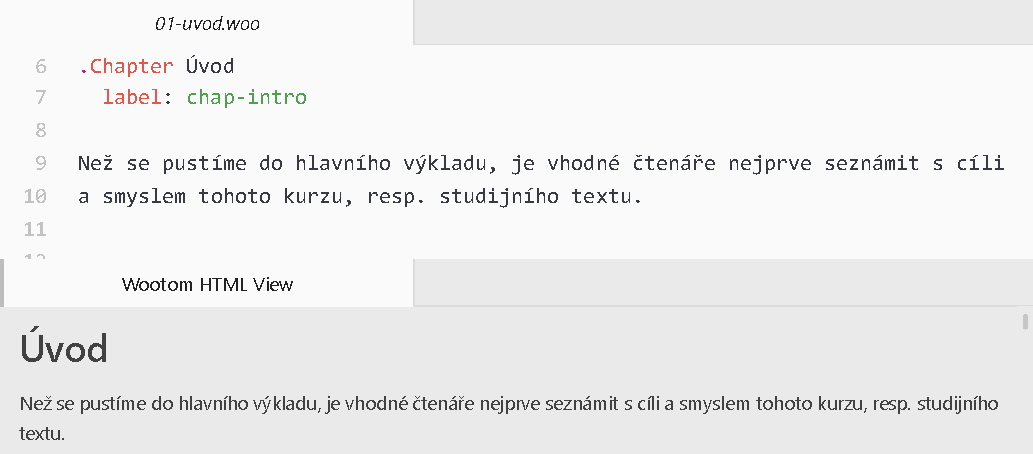
\includegraphics[width=1.0\textwidth]{content/realizace/nahled-pkm-kapitola}
 	\caption[Náhled části dokumentu]{Náhled části dokumentu ve zdroji studijního textu k BI-PKM \cite{pkm}}
    \label{zobrazeni-nahledu-pkm-kapitola}
\end{figure}

\#todo
